% @Author: Ren Qingjie
% @Date:   2017-05-28 23:06:23
% @Last Modified by:   Ren Qingjie
% @Last Modified time: 2017-05-29 02:00:09

% \documentclass{article}
\documentclass[xcolor=dvipsnames]{beamer}
\usecolortheme[named=Maroon]{structure}
\usetheme{Boadilla}
\usepackage{helvet}
\title[FOF]{Fund of Funds}
\author{Qi Zhou, Wang Zhe, Ren Qingjie}
\institute{School of Physics \& School of Economics, Peking University}



\begin{document}
\maketitle



\begin{frame}
	\begin{itemize}
		\item{In this part, we would explore the relationship between the fund market and the retirement market.}
		\item{The Fund of Funds is favoured by risk averter, especially for those who have retired.}
		\item{There might be cointegration relationships bewteen the two markets.}
	\end{itemize}
	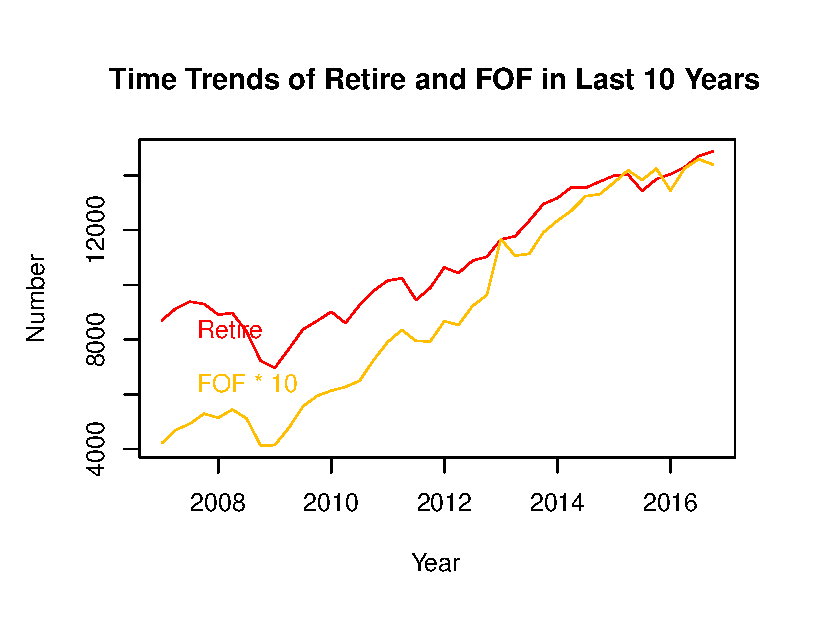
\includegraphics[scale=0.4]{3-1.eps}
	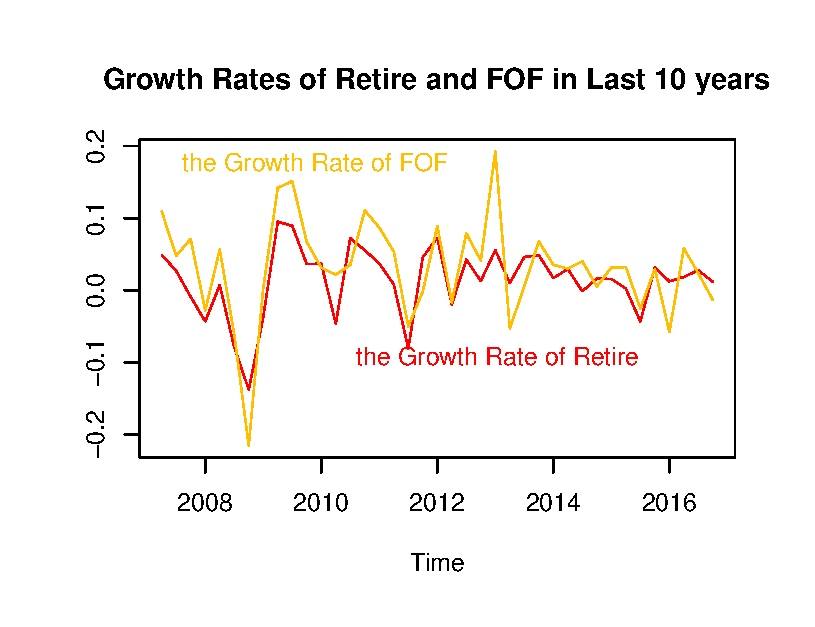
\includegraphics[scale=0.4]{3-2.eps}
\end{frame}


% 单位根检验 Unit Root Test
\begin{frame}{Unit Root Test}
	% \bigskip
	% 3 tests are employed here: \bold{ADF-Test}, \bold{KPSS-Test} , and \bold{PP-Test}
	3 tests are employed here: ADF-Test, KPSS-Test, and PP-Test (Phillips-Perron Test).

	Unit Root Test of Retire\\
	\par
	\begin{tabular}{|r |c |c |c| c|}
		\hline
		Test Method&Statistics & 10pct & 5pct & 1pct \\  \hline
		ADF & 1.64 &-1.61 & -1.95&-2.62 \\  \hline
		KPSS & 1.01 & 0.35 & 0.46 & 0.74 \\  \hline
		PP & 0.23 & *  &0.26 & *\\  \hline
	\end{tabular}
	\\
	\bigskip
	Unit Root Test of the Difference of Retire \\
	\begin{tabular}{|r |c |c |c| c|}
		\hline
		Test Method&Statistics & 10pct & 5pct & 1pct \\  \hline
		ADF & -2.31 &-1.61 & -1.95&-2.62 \\  \hline
		KPSS & 0.18 & 0.35 & 0.46 & 0.74 \\  \hline
		PP & 1.55 & *  &0.26 & *\\  \hline
	\end{tabular}	
	\\
	\bigskip
	\par
	Unit Root Test of FOF \\
	\begin{tabular}{|r |c |c |c| c|}
		\hline
		Test Method&Statistics & 10pct & 5pct & 1pct \\  \hline
		ADF & 2.53 &-1.61 & -1.95&-2.62 \\  \hline
		KPSS & 1.07 & 0.35 & 0.46 & 0.74 \\  \hline
		PP & -0.16 & *  &0.26 & *\\  \hline
	\end{tabular}
	\par
	Unit Root Test of difference of FOF \\
	\begin{tabular}{|r |c |c |c| c|}
		\hline
		Test Method&Statistics & 10pct & 5pct & 1pct \\  \hline
		ADF & -3.40 &-1.61 & -1.95&-2.62 \\  \hline
		KPSS & 0.11 & 0.35 & 0.46 & 0.74 \\  \hline
		PP & -40 & *  &0.26 & *\\  \hline
	\end{tabular}

\end{frame}
\begin{frame}{Unit Root Test}
	3 tests are employed here: ADF-Test, KPSS-Test, and PP-Test (Phillips-Perron Test). \\
	\begin{tabular}{|l| c| c| c|}
	\hline
	\textsc{Test} Method &  ADF   & KPSS &  PP   \\ \hline
	FOF 				 &  2.53  & 1.07 & -0.16 \\ \hline
	diff(FOF) 			 & -3.40  & 0.11 & 40 	 \\ \hline
	Retire 				 &  1.64  & 1.01 & 0.23  \\ \hline
	diff(Retire) 		 & -2.31  & 0.18 & 1.55  \\ \hline
	10pct 				 & -1.61  & 0.35 &   * 	 \\ \hline
	5pct 				 & -1.95  & 0.46 & 0.26  \\ \hline
	1pct 				 & -2.62  & 0.74 &   * \\ \hline

	\end{tabular}

\end{frame}


%  模型1, Model 1
\begin{frame}{Cointegration Relationship One}

\end{frame}


\begin{frame}{Error Correction Model One}
\end{frame}


% 模型2, Model 2
\begin{frame}{Cointegration Relationship Two}
\end{frame}


\begin{frame}{Error Correction Model Two}
\end{frame}


% 模型3, Model 3
\begin{frame}{Cointegration Relationship Three}
\end{frame}


\begin{frame}{Error Correction Model Three}
\end{frame}


\end{document}
